% Part: model-theory
% Chapter: interpolation
% Section: separation

\documentclass[../../../include/open-logic-section]{subfiles}

\begin{document}

\olfileid{mod}{int}{sep}

\olsection{فصل الـ\printtoken{P}{sentence}}

لا بد قبل برهان الاستيفاء من تمهيد. مستوفية
$!A$ و$!B$ هي !!a{sentence}~$!C$ تحقق $!A \Entails !C$
و$!C \Entails !B$. والشرط الأخير يكافئ، بالمقابلة،
$\lnot !B \Entails \lnot !C$. فإذا كانت !!^a{sentence}~$!C$
على هذه الصفة قلنا إنها \emph{تفصل} $!A$ عن $\lnot !B$.
فطلب مستوفية لـ$!A$ و$!B$ هو طلب !!a{sentence}
تفصل $!A$ عن $\lnot !B$. ونوسّع النظر الآن إلى جملة
تفصل \emph{مجموعتين} من الـ!!{sentence}s، ففي هذا
التعميم نفع للبرهان.

\begin{defn}
\emph{تفصل} جملة~$!C$ مجموعتي الجمل $\Gamma$ و$\Delta$ إذا وفقط إذا كان
$\Gamma \Entails !C$ و$\Delta \Entails \lnot !C$. وإذا لم توجد
!!{sentence} كهذه، كانت $\Gamma$ و$\Delta$ \emph{غير قابلتين للفصل}.
\end{defn}

ويبيّن الشكل علاقات الاحتواء بين فئات نماذج $\Gamma$ و$\Delta$ و$!C$:
\begin{figure}[h]
  \centering
  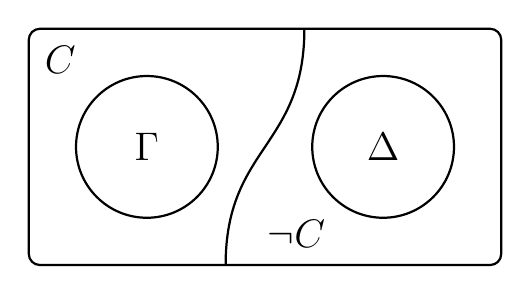
\begin{tikzpicture}[node distance=2cm, auto, thick]
    \draw [rounded corners] (0,0) -- (6,0) -- (6,3) -- (0,3) --  cycle;
    \draw (1.5,1.5) circle (0.9cm);
    \draw (4.5,1.5) circle (0.9cm);
    \path node at (1.5,1.5) {\Large $\Gamma$};
    \path node at (4.5,1.5) {\Large $\Delta$};
    \path node at (0.4,2.6) {\Large $\formula{C}$};
    \path node at (3.4,0.4) {\Large $\lnot \formula{C}$};
    \draw (2.5,0) .. controls (2.5,1.5) and (3.5,1.5) .. (3.5,3);
  \end{tikzpicture}
  \caption{$!C$ تفصل $\Gamma$ عن $\Delta$}
  \ollabel{fig:sep}
\end{figure}


\begin{lem}\ollabel{lem:sep1}
افترض أن $\Lang{L}_0$ هي اللغة التي تحتوي كل !!{constant} و!!{function}
و!!{predicate} (عدا~$\doteq$) يقع في $\Gamma$ و$\Delta$ \emph{معًا}،
ولتكن $\Lang{L}'_0$ ناتجة بإضافة عدد لا نهائي من الـ!!{constant}s الجديدة
$\Obj c_n$، حيث $n \ge 0$. إذا كانت $\Gamma$ و$\Delta$ غير قابلتين
للفصل في $\Lang{L}_0$، فهما غير قابلتين للفصل في $\Lang{L}'_0$ أيضًا.
\end{lem}

\begin{proof}
لنفرض خلاف المطلوب: أن $\Gamma$ و$\Delta$ تفصلهما
جملة في $\Lang{L}'_0$. فيكون
$\Gamma \Entails \Subst{!C}{c}{x}$ و
$\Delta \Entails \lnot \Subst{!C}{c}{x}$ لبعض
$!C \in \Lang{L}_0$، حيث $c$~!!{constant} جديد.
ونقتصر على هذه الحال؛ أما ما ينتج من $!C$ باستعمال أكثر
من !!{constant} جديد فبرهانه نظيرها.
بالتراص نجد جزءًا \emph{منتهيًا} $\Gamma_0$ من $\Gamma$
وجزءًا منتهيًا $\Delta_0$ من $\Delta$، بحيث
$\Gamma_0 \Entails \Subst{!C}{c}{x}$ و
$\Delta_0 \Entails \lnot \Subst{!C}{c}{x}$.
نجعل $!G$ اقتران الـ!!{formula}s التي في $\Gamma_0$،
و$!H$ اقتران الـ!!{formula}s التي في $\Delta_0$، فنحصل على
\begin{align*}
  !G & \Entails \Subst{!C}{c}{x}, & !H  \Entails \lnot \Subst{!C}{c}{x}.
\end{align*}
من الجهة الأولى نستنتج بالتعميم $!G \Entails \lforall[x][!C]$.
ومن الجهة الثانية نستنتج بالمقابلة
$\Subst{!C}{c}{x} \Entails \lnot !H$، فيلزم
$\lforall[x][!C] \Entails \lnot !H$.
وبمقابلة أخرى نحصل على $!H \Entails \lnot \lforall[x][!C]$.
ثم تقضي الرتابة بأن
\begin{align*}
  \Gamma &\Entails \lforall[x][!C], &
  \Delta & \Entails \lnot \lforall[x][!C],
\end{align*}
فتكون $\lforall[x][!C]$ فاصلةً بين~$\Gamma$ و$\Delta$ في $\Lang{L}_0$، خلاف الفرض.
\end{proof}

\begin{lem}\ollabel{lem:sep2}
افترض أن $\Gamma \cup \{ \lexists[x][!S] \}$ و$\Delta$ غير قابلتين
للفصل، وأن $c$~!!{constant} جديد لا يقع في $\Gamma$ أو $\Delta$ أو
$!S$. عندئذ تكون
$\Gamma \cup \{ \lexists[x][!S], \Subst{!S}{c}{x} \}$ و$\Delta$
غير قابلتين للفصل أيضًا.
\end{lem}

\begin{proof}
لنفرض أن $!C$ تفصل
$\Gamma \cup \{\lexists[x][!S], \Subst{!S}{c}{x}\}$ عن $\Delta$،
مع أن $\Gamma \cup \{\lexists[x][!S] \}$ و$\Delta$
غير قابلتين للفصل. والبحث على حالين:
\begin{enumerate}
\item إن لم يقع $c$ في $!C$، كانت
  $\Gamma \cup \{\lexists[x][!S], \lnot!C \}$ قابلة للإرضاء؛
  وإلا فصلت $!C$~$\Gamma \cup \{\lexists[x][!S] \}$ عن $\Delta$.
  ولنا أن نضيف $\Subst{!S}{c}{x}$ ونبقي الإرضاء، بتأويل
  الثابت الجديد بشاهد الوجود. فلا تفصل $!C$
  المجموعة $\Gamma \cup \{ \lexists[x][!S], \Subst{!S}{c}{x} \}$
  عن $\Delta$، خلاف الفرض.
\item وإن وقع $c$ في $!C$، كتبنا $!C$ على الصورة
  $\Subst{!C}{c}{x}$. وعندئذ
  \[
  \Gamma \cup \{ \lexists[x][!S], \Subst{!S}{c}{x}\} \Entails \Subst{!C}{c}{x},
  \]
  فنستنتج $\Gamma, \lexists[x][!S] \Entails \lforall[x][(!S \lif !C)]$
  بمبرهنة الاستنباط والتعميم، ثم
  $\Gamma \cup \{ \lexists[x][!S] \} \Entails \lexists[x][!C]$.
  وفي الجهة الأخرى $\Delta \Entails \lnot \Subst{!C}{c}{x}$،
  فيعطي التعميم $\Delta \Entails \lnot \lexists[x][!C]$.
  فتكون $\Gamma \cup \{\lexists[x][!S] \}$ و$\Delta$
  قابلتين للفصل، وهذا تناقض.
\end{enumerate}
\end{proof}

\end{document}
